%%%%%%%%%%%%%%%%%%%%%%%%%%%%%%%%%%%%%
%% Supporting Information
%% (Optional)
%%%%%%%%%%%%%%%%%%%%%%%%%%%%%%%%%%%%%
% OVERVIEW
%
% Please note that all supporting information will be peer reviewed with your manuscript.
% In general, the purpose of the supporting information is to enable
% authors to provide and archive auxiliary information such as data
% tables, method information, figures, video, or computer software,
% in digital formats so that other scientists can use it.

% The key criteria are that the data:
% 1. supplement the main scientific conclusions of the paper but are not essential to the conclusions (with the exception of
%    including data so the experiment can be reproducible);
% 2. are likely to be usable or used by other scientists working in the field;
% 3. are described with sufficient precision that other scientists can understand them, and
% 4. are not exe files.
%

% All Supporting text and figures should be included in this document.

% Data sets, large tables, movie files,
% and audio files should be uploaded separately, following AGU naming
% conventions. Include their captions in this document and list the
% file name with the caption. You will be prompted to upload these
% files on the Upload Files tab during the submission process, using
% file type “Supporting Information (SI)”

\documentclass{agujournal2018}

% Please type in the journal name: \journalname{<Journal Name>}
% ie,
\journalname{JGR-Space Physics}

%% Choose from this list of Journals:
%
% Journal of Geophysical Research
% JGR-Biogeosciences
% JGR-Earth Surface
% JGR-Planets
% JGR-Solid Earth
% JGR-Space Physics
% Global Biochemical Cycles
% Geophysical Research Letters
% Paleoceanography
% Radio Science
% Reviews of Geophysics
% Tectonics
% Space Weather
% Water Resource Research
% Geochemistry, Geophysics, Geosystems
% Journal of Advances in Modeling Earth Systems (JAMES)
% Earth's Future
% Earth and Space Science

\usepackage[round, sort, numbers, authoryear]{natbib}
\usepackage{amsmath}
\usepackage{amsfonts}
\PassOptionsToPackage{hyphens}{url}
\usepackage[colorlinks=true]{hyperref}
\usepackage{multirow}
\usepackage[]{changes}


\begin{document}

\renewcommand{\thetable}{S\arabic{table}}
\renewcommand{\thefigure}{S\arabic{figure}}

%% This command needs article title as argument to \supportinginfo{}:
\supportinginfo{Probabilistic Geomagnetic Storm Forecasting via Deep Learning}

\authors{Adrian Tasistro-Hart\affil{1,2}, Alexander Grayver\affil{1}, Alexey Kuvshinov\affil{1}}

\affiliation{1}{Institute of Geophysics, ETH Z\"urich, Sonneggstrasse 5, 8092 Z\"urich, Switzerland}
\affiliation{2}{Department of Earth Science, University of California, Santa Barbara, CA 93106, USA}


%% Corresponding Author
%(include name and email addresses of the corresponding author.  More
%than one corresponding author is allowed in this Word file and for
%publication; but only one corresponding author is allowed in our
%editorial system.)  

\correspondingauthor{Adrian Tasistro-Hart}{adrian\_tasistro-hart@ucsb.edu}

%% ------------------------------------------------------------------------ %%
%
%  TEXT
%
%% ------------------------------------------------------------------------ %%

\section*{Contents}
%%%Remove or add items as needed%%%
\begin{enumerate}
\item Text S1 to S6
\item Figures S1 to S9
\item Table S1
\end{enumerate}

%%
%% DATA GAP HANDLING
%%
\section*{Text S1: Data continuity and gap handling}\label{sec:datahandling}

% OMNI
\subsection*{OMNI data}\label{sec:OMNIsupp}
We accessed the low-resolution OMNI dataset via the \href{https://omniweb.gsfc.nasa.gov/ow.html}{OMNIWeb interface}. Within the OMNI data, all gaps of 72 hours or less were filled via linear interpolation.

% CME
\subsection*{CME data}
The CME data were taken from the \href{https://cdaw.gsfc.nasa.gov/CME_list/}{SOHO LASCO CME catalog}.

Given that this project works with hourly data and multiple CMEs can occur within the same hour, the CME with the largest energy was taken in the cases when multiple CMEs did occur within an hour. Additionally, many events in the catalogue did not have all data fields filled, hence we used only the events for which all data were reported.

% GOES
\subsection*{GOES data}\label{sec:GOESsupp}

The GOES x-ray flux data are provided by \href{https://satdat.ngdc.noaa.gov/sem/goes/data/avg}{NOAA} with one minute averaging. All the available files were downloaded for which primary and secondary satellites were specified and data from the satellite recommended by this relevant \href{https://www.ngdc.noaa.gov/stp/satellite/goes/doc/GOES\_XRS\_readme.pdf}{NOAA document} was taken. These minute data were averaged in hourly bins to generate time series consistent with the other data sources. No gap exceeded 72 hours, and all gaps were interpolated linearly.

% UNCERTAINTY IN MODEL
\section*{Text S2: Uncertainty in model parameters}\label{sec:variational_intro}
One major paradigm of learning uncertainty in neural networks is to represent the network weights, or some internal aspect of the network, probabilistically. One of the first implementations was proposed by \cite{Blundell2015}, who describe an architecture in which all of the network weights and biases are represented as distributions, and the problem becomes learning the parameters of those distributions. To achieve this, \cite{Blundell2015} outline a variational Bayesian framework. Variational refers to the fact that the true distribution over network weights is approximated by some simpler distribution, and Bayesian refers to the representation of this conditional distribution via Bayes' rule.

% In the ideal world, the goal would be to obtain perfect knowledge about $p(\mathbf{w} \vert \mathbf{x}, \mathbf{y})$, which is a posterior distribution over the network weights (and biases) given the observed data. While we could sample from this distribution using techniques like Markov-chain Monte-Carlo (MCMC), in general we cannot learn this probability density for all network weights in reasonable time. Instead, the goal is to learn a variational posterior $q(\mathbf{w} \vert \theta)$, parameterized by $\theta$, which has a much simpler form than the unknown true posterior. Since we seek a variational posterior that is as similar as possible to the true posterior, we need to define a metric of misfit between the distributions. The Kullback-Leibler divergence is a commonly chosen measure, and we thus have the following optimization problem:

% \begin{equation}
% \underset{\theta}{\text{min}} \; D_{KL}( q(\mathbf{w} \vert \theta) \Vert p(\mathbf{w} \vert \mathbf{x}, \mathbf{y})) = \underset{\theta}{\text{min}} \; \int_\mathbf{w} q(\mathbf{w} \vert \theta)\,\log\frac{q(\mathbf{w} \vert \theta)}{p(\mathbf{w} \vert \mathbf{x}, \mathbf{y})}\,d\mathbf{w}
% \end{equation}

% Furthermore, since we do not have access to the true posterior to compute this divergence, we represent it via Bayes' theorem $p(\mathbf{w} \vert \mathbf{x}, \mathbf{y}) = \frac{p(\mathbf{x}, \mathbf{y} \vert \mathbf{w})\, p(\mathbf{w})}{p(\mathbf{x}, \mathbf{y})} $, and the minimization becomes:

% \begin{eqnarray} 
% \underset{\theta}{\text{min}} \; \int_\mathbf{w} q(\mathbf{w} \vert \theta)\,\log\frac{q(\mathbf{w} \vert \theta)\, p(\mathbf{x}, \mathbf{y})}{p(\mathbf{x}, \mathbf{y} \vert \mathbf{w})\, p(\mathbf{w})}\,d\mathbf{w} =  \nonumber \\
% \begin{split} 
% \underset{\theta}{\text{min}} \; \int_\mathbf{w} q(\mathbf{w} \vert \theta)\,\log q(\mathbf{w} \vert \theta) \, d\mathbf{w} + \int_\mathbf{w} q(\mathbf{w}\vert\theta) \,\log{p(\mathbf{x}, \mathbf{y})} \, d\mathbf{w} \nonumber \\ 
% - \int_\mathbf{w} q(\mathbf{w} \vert \theta)\,p(\mathbf{w}) \, d\mathbf{w} - \int_\mathbf{w} q(\mathbf{w} \vert \theta)\, p(\mathbf{x}, \mathbf{y} \vert \mathbf{w}) \, d\mathbf{w} =
%  \end{split}  \nonumber \\
% \underset{\theta}{\text{min}} \; \mathbb{E}_q \left[ \log q(\mathbf{w} \vert \theta)\right] - \mathbb{E}_q \left[ \log p(\mathbf{w}) \right] - \mathbb{E}_q \left[ \log p(\mathbf{x}, \mathbf{y} \vert \mathbf{w})\right]  \label{eq:variational}
% \end{eqnarray}

% where we ignore the $\int_\mathbf{w} q(\mathbf{w}\vert\theta) \,\log{p(\mathbf{x}, \mathbf{y})} \, d\mathbf{w} = p(\mathbf{x}, \mathbf{y})$ term because it does not depend on $\theta$. 

The cost function in this framework (Equation~\ref{eq:variational} depends only on the variational posterior, a prior over the weights (which we must specify), and a likelihood term dependent on the data. \cite{Blundell2015} propose a Gaussian mixture $ p(\mathbf{w}) = \prod_i \pi \, \mathcal{N}(\mathbf{w}_i \vert 0, \sigma_1^2) + (1-\pi)\,\mathcal{N}(\mathbf{w}_i \vert 0, \sigma_2^2)$ for the prior, which we also utilize. This likelihood term is captured by a NN. Because the expectations are taken over the variational posterior, we can approximate them simply by sampling weights from their variational posteriors for given $\theta$, and then we can update $\theta$ by differentiating the total loss against $\theta$. This approach requires us to specify a functional form for $p(\mathbf{x}, \mathbf{y} \vert \mathbf{w})$, which effectively captures the level of anticipated noise in the training data.

\begin{equation}
    \underset{\theta}{\text{min}} \; \mathbb{E}_q \left[ \log q(\mathbf{w} \vert \theta)\right] - \mathbb{E}_q \left[ \log p(\mathbf{w}) \right] - \mathbb{E}_q \left[ \log p(\mathbf{x}, \mathbf{y} \vert \mathbf{w})\right]  \label{eq:variational}
\end{equation}

This approach hinges on the choice of a simple variational posterior, and \cite{Blundell2015} suggest a Gaussian posterior over the weights. Since the Gaussian is a two-parameter model, this sort of architecture effectively double the number of parameters per weight, since the network learns a mean and a variance for each weight. 

Given that the numerical differentiation can easily be done by TensorFlow, what remains is only to add the so-called``KL-losses'' $ \mathbb{E}_q \left[ \log q(\mathbf{w} \vert \theta)\right] - \mathbb{E}_q \left[ \log p(\mathbf{w}) \right]$ to the negative log-likelihood loss of the data given weights sampled from the variational posterior while ensuring that the learnable parameters in the network are the $\theta$ parameterizing the variational posterior distributions over the weights. With a trained the network, arbitrarily many outputs can be sampled for a given input by sampling from the variational posterior over the weights, effectively simulating output from an ensemble of models. Then, statistics such as confidence intervals can be computed from this output.

This approach to probabilistic neural networks did not result in meaningful probabilistic forecasts for Est (Figure~\ref{fig:weight_uncertainty}). Instead, the variational approach ended up learning a well-constrained posterior over the network weights, indicating that the network was quite confident that it had learned the optimal model. The confidence interval constructed from a Monte Carlo suite of models drawn from the variational posterior over the weights is barely visible around the mean posterior forecast, even though this confidence interval almost never contains the observed Est values. This approach simply demonstrates that the optimal model is confidently known by the network.

\begin{figure}[htbp]
  \centering
  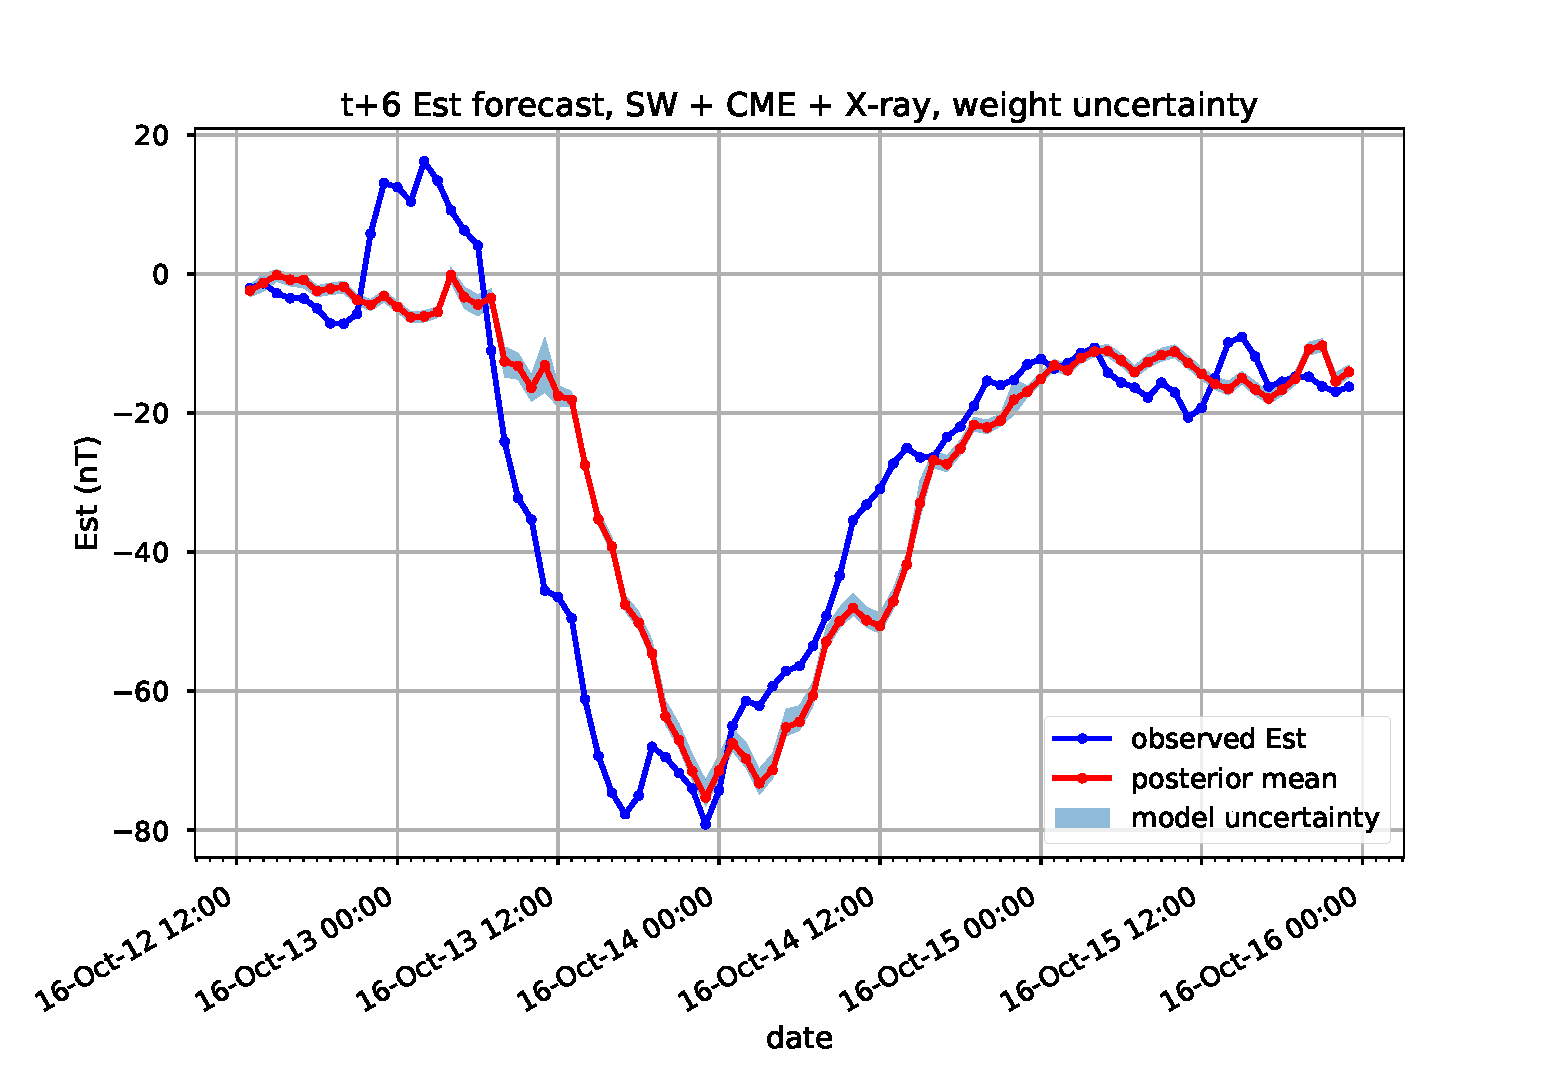
\includegraphics[width=0.8\textwidth]{figures/supplement/Est_forecast_SWCMEXray_weightuncertainty_t+6_storm1.pdf} 
  \caption{Model output for at 6 hour ahead forecast from the probabilistic network modeling uncertainty over network weights. The confidence interval was computed by sampling several thousand weights from the trained network and taking the 2.5-97.5\% interval of output values. }
  \label{fig:weight_uncertainty}
\end{figure}


%%
%% OUTPUT DISTRIBUTION
%%
\section*{Text S3: Output distribution selection}

Basic statistics of Est observations can inform the choice of output distribution. For instance, the  empirical histogram of Est shows an asymmetry defined by a large tail at negative values (Figure~\ref{fig:est_stats}B). Symmetric two-parameter distributions like the Gaussian and Laplace distributions fail to capture this asymmetry, and the Gaussian distribution furthermore fails to capture the heavy negative tail. These results are demonstrated by the quantile-quantile plots, which show that the Gumbel distribution is most appropriate for modeling the empirical distribution of Est (Figure~\ref{fig:est_stats}A). The Gumbel distribution is from the family of generalized extreme value distributions often used to model phenomena with heavy tails such as earthquakes or flooding events. In this sense, the distribution of Est captures the extreme value nature of geomagnetic storms and motivates the utilization of the Gumbel distribution as an output distribution for probabilistic forecasting of Est.

\begin{figure}[htbp]
   \centering
   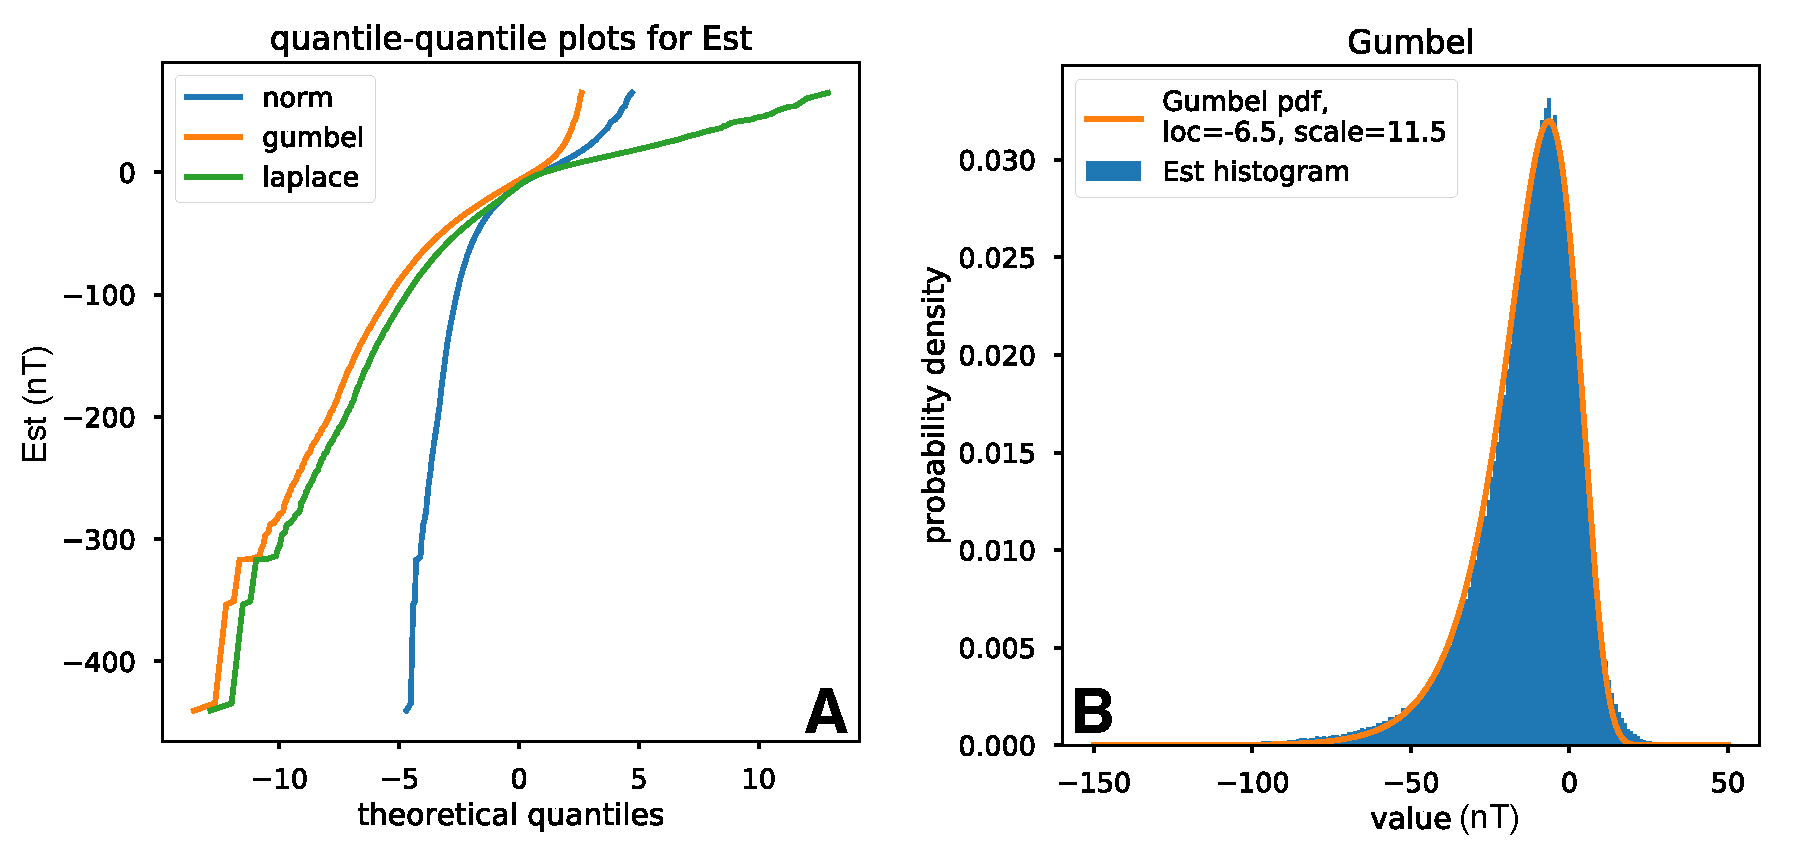
\includegraphics[width=1.0\textwidth]{figures/supplement/est_stats.pdf} % requires the graphicx package
   \caption{(A) Quantile-quantile plots for Est for three two-parameter distributions. The Gumbel distribution is closest to linear. (B) Empirical histogram of Est and a well-fitting Gumbel probability density showing how the asymmetry of the Gumbel distribution is capable of capturing the long tail of negative Est values.}
   \label{fig:est_stats}
\end{figure}

However, while the marginal distribution of Est might be well-approximated by a Gumbel distribution, the forecast itself is a much more complicated distribution conditioned on the time history of the input data, neural network weights and biases, and the internal memory of the LSTM cell. The nature of this conditional output distribution is unknown. While it could be framed in a Bayesian sense, where the prior could be specified as a Gumbel distribution, the evidence and likelihood terms in this framework are not at all obvious to construct. Instead, we argue for regularization of the cost function, which can be heuristically motivated. This regularization is necessary because the choice of output distribution and cost function strongly impact the qualitative nature of network output (Figure~\ref{fig:storm4_forecast}) and forecast reliability (Figure~3 in manuscript).

We considered three cases:
\begin{enumerate}
    \item Gumbel output distribution with Gumbel as likelihood cost function.
    \item Gaussian output distribution with Gaussian as likelihood cost function.
    \item Gaussian output with regularized Gaussian as likelihood cost function.
\end{enumerate}
The first two cases follow the paradigm that the output distribution simultaneously serves as the likelihood distribution that is the cost function in this probabilistic framework. Output from each of these is shown for a storm in Figure~\ref{fig:storm4_forecast}, and the overall reliability of these networks demonstrates that the third, regularized architecture is most reliable (Figure~3 in main manuscript).

\begin{figure}[htbp]
  \centering
  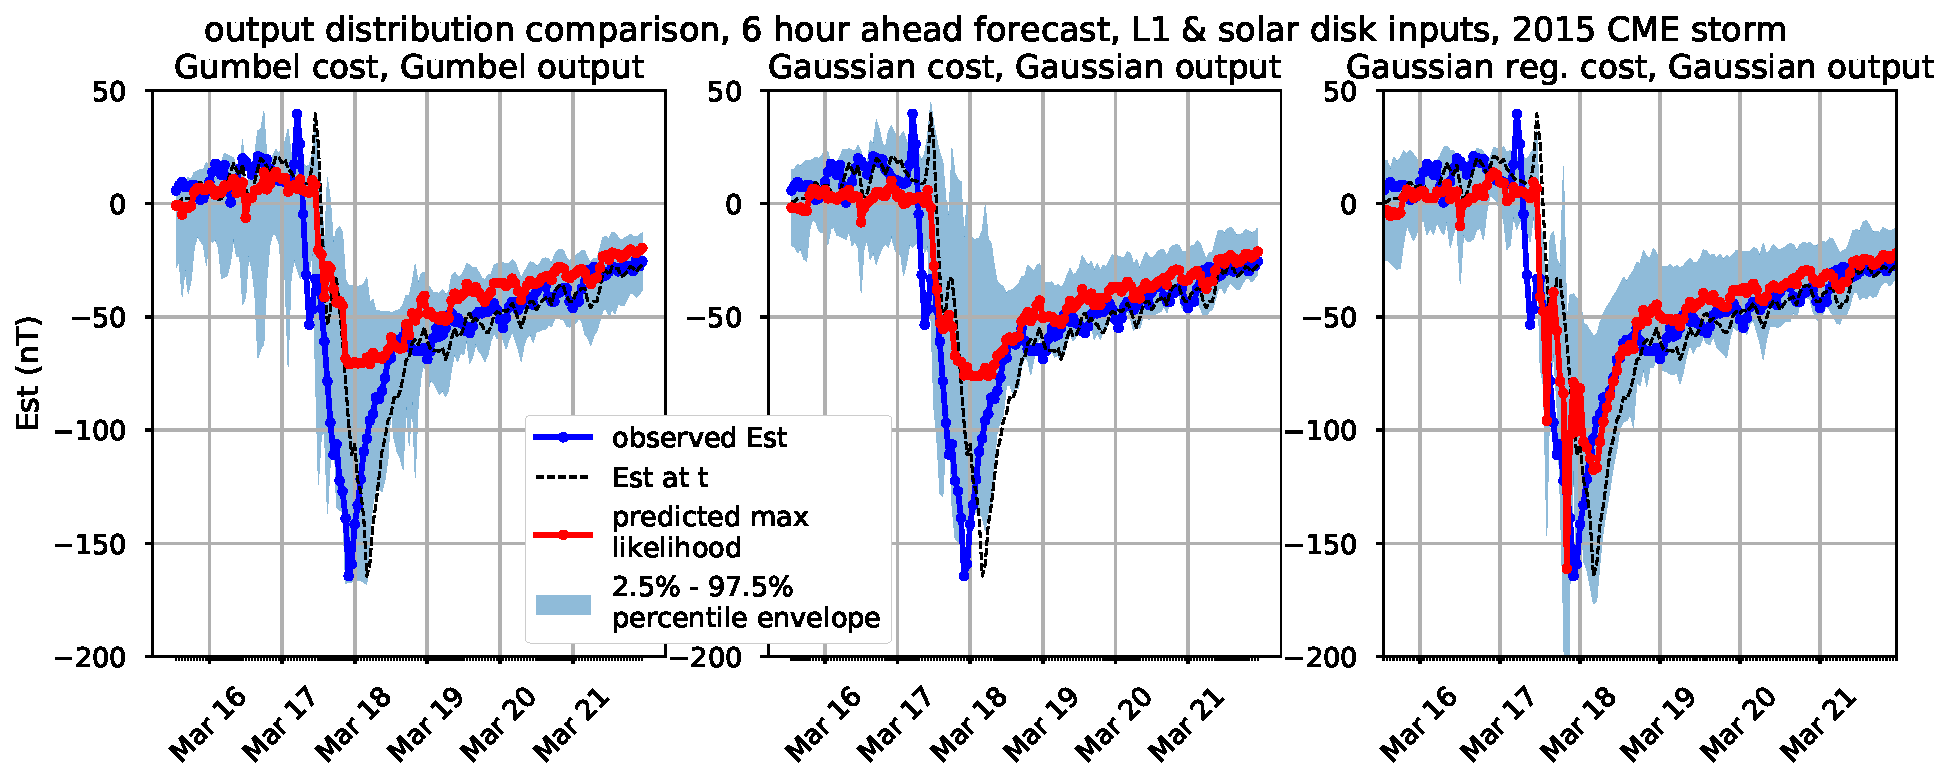
\includegraphics[width=1.0\textwidth]{figures/supplement/est_forecast_distcompare_storm4.pdf} 
  \caption{Network output for a 6 hour ahead Est forecast for three different cost functions. Left: output over Gumbel distributions with the Gumbel likelihood cost (Equation~\ref{eq:gumbelcost}). Middle/Right: both networks learned Gaussian outputs, but the right plot shows output for the network that utilized the regularized Gaussian cost function (Equation~\ref{eq:gaussian_mod}), while the middle one utilized the basic Gaussian likelihood function (Equation~\ref{eq:gaussian}). All networks were trained on data from both the solar disk (x-ray fluxes, CMEs) as well as solar wind observations from the L1 point.}
  \label{fig:storm4_forecast}
\end{figure}

The cost functions corresponding to these cases are negative log-likelihoods, whose expressions are
\begin{eqnarray}
	C_{\mathrm{Gumbel}}(y, \mu, \sigma) =& \log\,\sigma - \frac{y-\mu}{\sigma} + e^{\frac{y-\mu}{\sigma}} \label{eq:gumbelcost} \\
	C_{\mathrm{Gaussian}}(y, \mu, \sigma) =& \log\left(\sqrt{2\,\pi}\,\sigma \right) + \frac{\left(y-\mu \right)^2}{2\,\sigma^2} \label{eq:gaussian}\\
	C_{\mathrm{Gaussian,\, regularized}}(y, \mu, \sigma) =& \log\left(\sqrt{2\pi}\,\sigma \right) + \frac{\left(y-\mu \right)^2}{2\,\sigma^2} +  \alpha\,\left(y-\mu \right)^2 + \beta\,\frac{1}{\sigma^2} \label{eq:gaussian_mod}
\end{eqnarray}

The cost functions in Equations~\ref{eq:gumbelcost} and~\ref{eq:gaussian}, which are both negative log-likelihoods, produced networks that would not forecast mean values less than -100 nT. This effect is quite apparent in the first panel of Figure~\ref{fig:storm4_forecast}, where the Gumbel network forecasts storm main phase values at most -75 nT despite observed values exceeding -150 nT. Given that this network is generating a 6 hour ahead forecast, observations of Est from 6 hours ago should contribute information about reasonable magnitudes for the current forecast, meaning that once observed values decreased beyond -75 nT, one might expect the network to forecast more negative values if it perceives the storm to be continuing. However, this is not the case for the storm shown, during which Est exceeded -75 nT for roughly 20 hours. What is apparent is that instead of moving the output distribution location, the network favored increasing the output uncertainty, in general capturing the observed range of variability within the 95\% confidence interval. While this result demonstrates that the network is aware of its forecast uncertainty during the main phase of the storm, the inability of the network to move its maximum likelihood estimate to forecast large storm magnitudes diminishes its operational reliability. The corresponding reliabilities demonstrate the reduced utility of the probabilistic forecasts for large storm amplitudes from the Gaussian and Gumbel networks: while they are quite reliable at smaller Est thresholds, forecasting Est beyond -75~nT becomes less reliable.

The structure of the cost functions for a given true Est value of -150~nT (Figure~\ref{fig:costs}) shows why the unregularized networks favor expanding uncertainty rather than shifting the central value for the forecast: the cost functions are much less sensitive to forecasted $\mu$ if the forecasted $\sigma$ is large, meaning that the network will tend to learn to increase $\sigma$ without having a strong incentive to learn a reasonable $\mu$. Thus, the idea to regularize is motivated by the desire to incentivize the network to learn more reasonable estimates for $\mu$. A simple way to include this incentive is to add another least squares cost that is not normalized by the forecasted uncertainty, as shown in Equation~\ref{eq:gaussian_mod}, where the quantity $\alpha$ is a new hyper-parameter that dictates the strength of this regularization. 

This additional cost forces the network to learn more reasonable forecasts for $\mu$ while still allowing it to change $\sigma$ quite freely for a given $\mu$. As can be seen in Figures~\ref{fig:storm4_forecast} and 3 (in manuscript), this regularization term significantly improves the forecast. The maximum likelihood forecast more closely overlaps the observed Est values, and the forecast uncertainty still exhibits meaningful behavior, with large uncertainties associated with storm arrivals and smaller uncertainties during storm recovery and quiet times. 

We also add a second regularizing term, $\beta\,\frac{1}{\sigma^2}$, which permits adjustment of the forecasted uncertainty. Positive values of $\beta$ penalize smaller forecast uncertainties, whereas negative values of $\beta$ encourage smaller forecast uncertainties.

\begin{figure}[htbp]
  \centering
  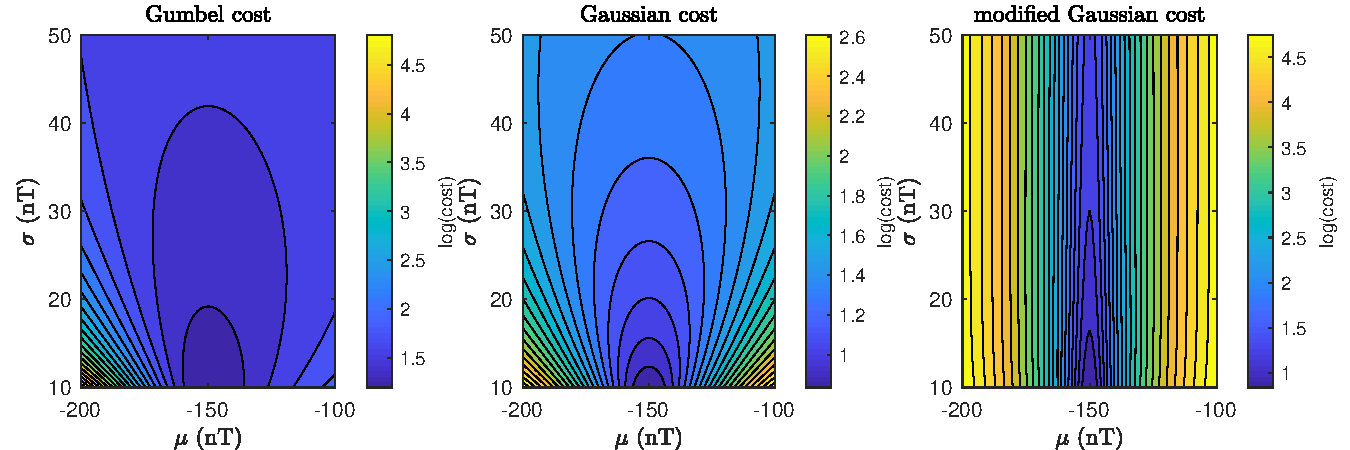
\includegraphics[width=1.0\textwidth]{figures/supplement/costs.pdf} 
  \caption{Cost functions for an observed output of $y=-150$ nT, with each panel corresponding to the cost functions used to train the networks whose output is shown in Figures~\ref{fig:storm4_forecast}. Note that the contours show the logarithm of the cost functions.}
  \label{fig:costs}
\end{figure}

%%
%% LEARNING PARAMETERS
%%
\section*{Text S4: Learning parameters}

This section briefly lists all other learning parameters used during training of the neural networks. The optimizer of choice is the so-called ``adam'' optimizer, which uses both momentum (i.e., memory of the previous update direction), and scaling by the inverse of the second moment of the gradient to generate first order updates in stochastic gradient descent optimization \citep{Kingma2014adam}. This optimizer has three hyperparameters, and the only one that was changed is the step-size multiplier. The value of this parameter was varied between 0.001 and 0.005. All networks were trained with batch sizes of 1000 hours, meaning that the trained LSTM cells developed memories relevant to processes operating on the timescale of months, which is more than enough for learning storm-scale dynamics on the timescales of days to weeks. Networks were trained over 1000-2000 epochs, where an epoch reflects one entire pass through the training dataset. We selected $\alpha=0.1$ and $\beta=1$ for the regularizing coefficient values in Equation~\ref{eq:gaussian_mod}.

%%
%% SW vs SW+CME+XRAY
%%
\section*{Text S5: Forecast accuracy sensitivity to input data}

In order to assess the benefit of incorporating observations from the solar disk, we trained two separate networks to generate probabilistic forecasts for Est: one network was trained on both data from the solar disk and solar wind observations from the L1 point (i.e., utilizing the GOES, CME, and OMNI data), and the second network was trained only on the solar wind observations from the L1 point (i.e., utilizing only the OMNI data). Both networks had identical architectures that differed only by the dimensionalities of the weights and biases necessary to accommodate the differing input dimensionalities.

This section demonstrates that utilizing observations of the solar disk in addition to observations from the L1 point as input data, forecasting of storm main phase timing and amplitude does not significantly improve, although the estimated of the uncertainty envelope becomes more reliable (Figures \ref{fig:storm1_both}-\ref{fig:storm1_l1}), especially for multiple hours ahead forecast. Nevertheless, more opportunities remain for developing neural network architectures capable of utilizing sparse, impulse-like solar disk observations.

\begin{figure}[htbp]
   \centering
   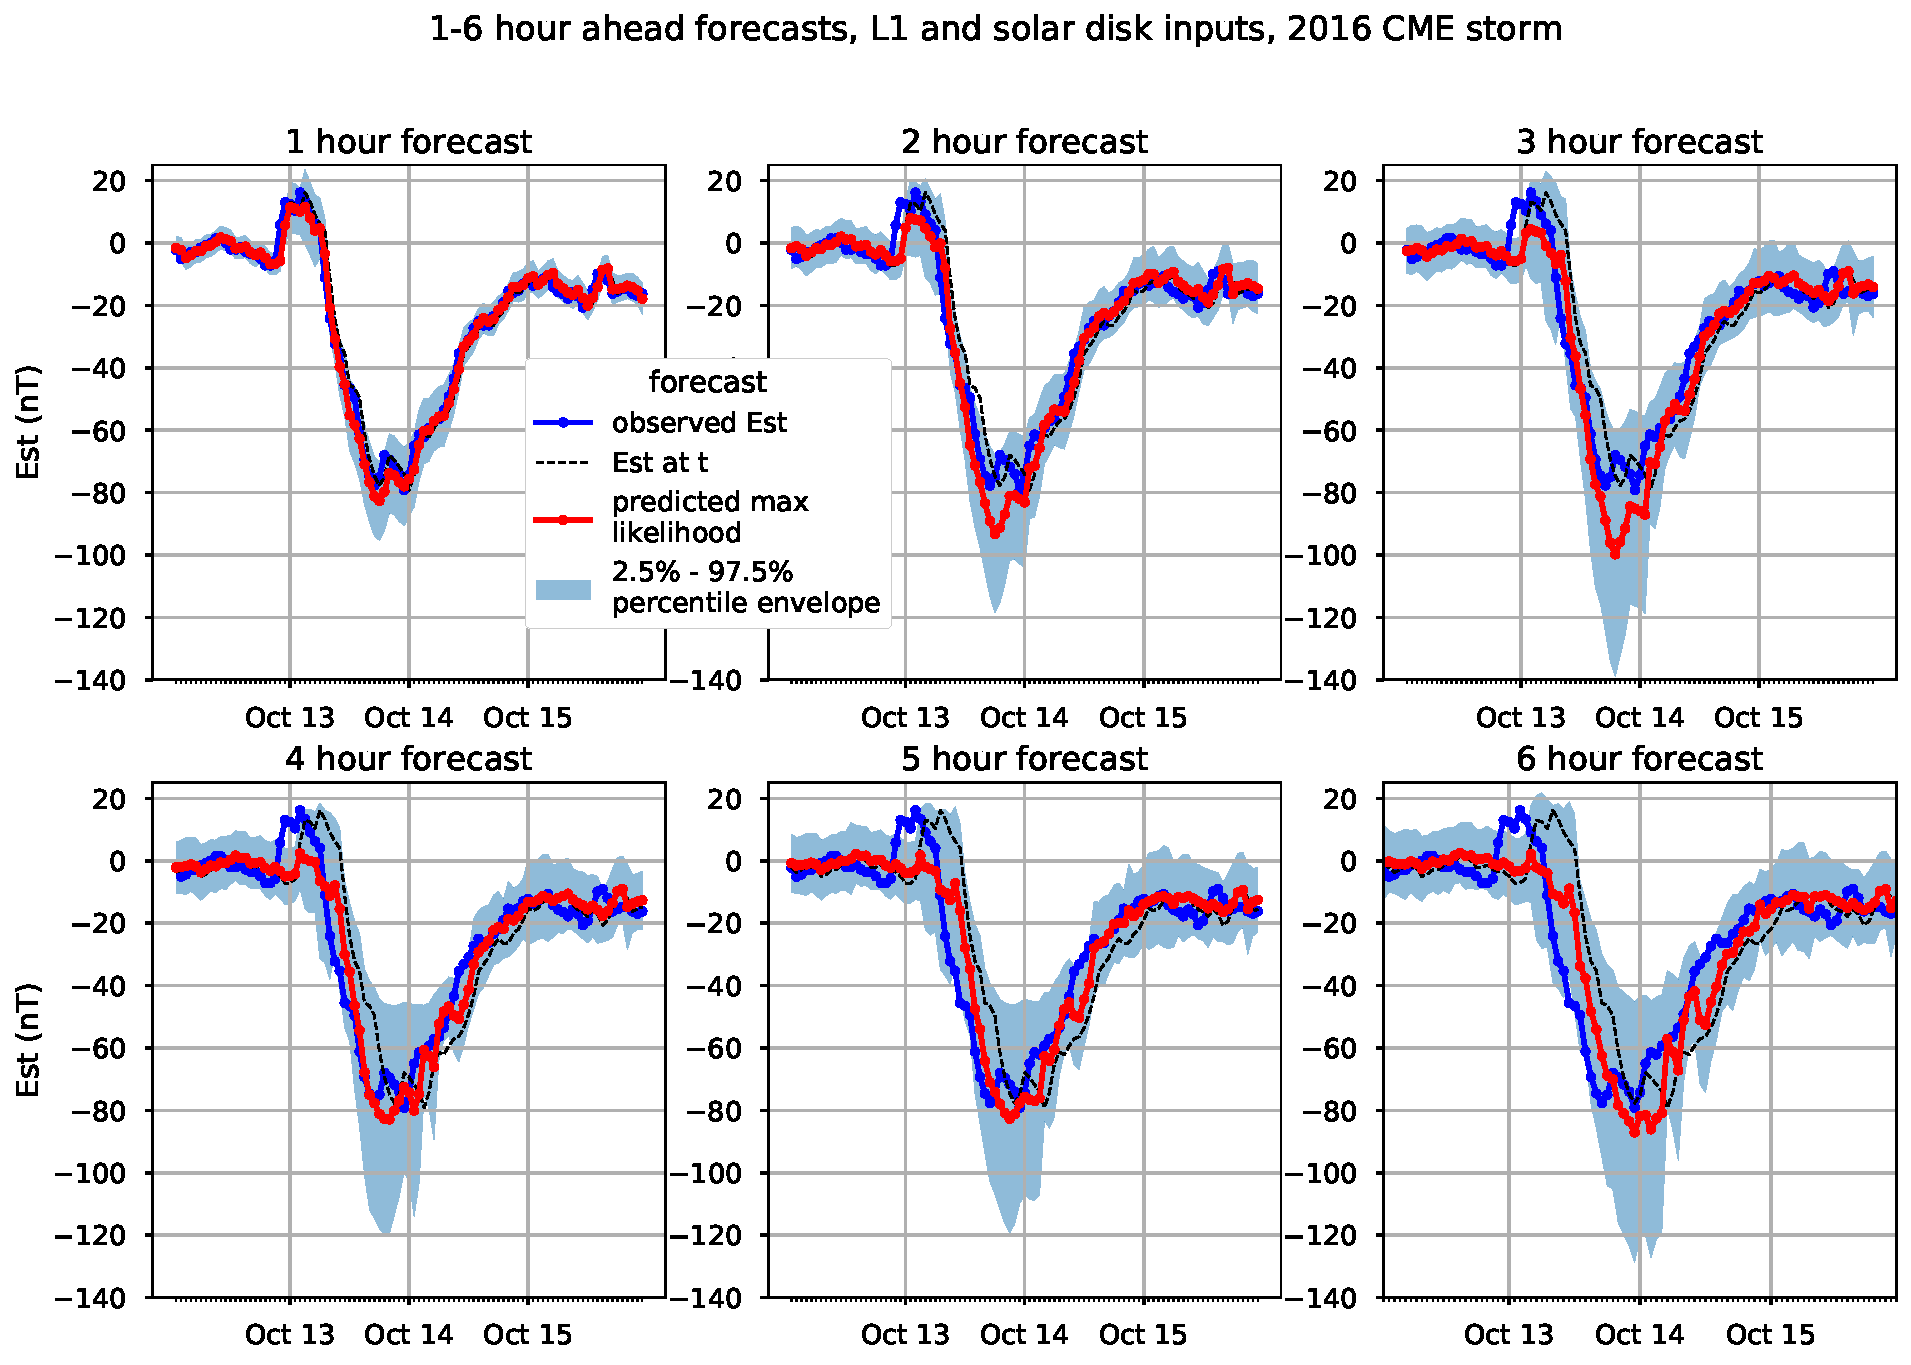
\includegraphics[width=1\textwidth]{figures/supplement/est_forecast_1-6_hour_L1&solardisk_storm1.pdf}
   \caption{1-6 hour ahead forecasts for the 2016 CME storm for the networks with observations from both the solar disk and L1 point as input.}
   \label{fig:storm1_both}
\end{figure}

\deleted{For both networks, storm onset remains difficult to predict, with the network not recognizing that a storm has begun until it receives as input the storm onset from the L1 point (Figures~\ref{fig:storm1_both} \& \ref{fig:storm1_l1}). Once the networks have felt the storm onset, however, they both dramatically expand uncertainty in their forecasts. The networks with only L1 inputs expand uncertainty more during the storm main phase and less during recovery and quiet times compared to the networks with both L1 and solar disk inputs, resulting in the observed reliability curves that demonstrate reduced reliability for low amplitude storms but slightly higher reliability for larger amplitude storms (Figure~\ref{fig:reliability_input}). For probable, high amplitude storms, then, the networks with only L1 inputs are slightly more reliable, while for smaller amplitude storms the networks with both L1 and solar disk inputs are more reliable.}

\begin{figure}[htbp]
   \centering
   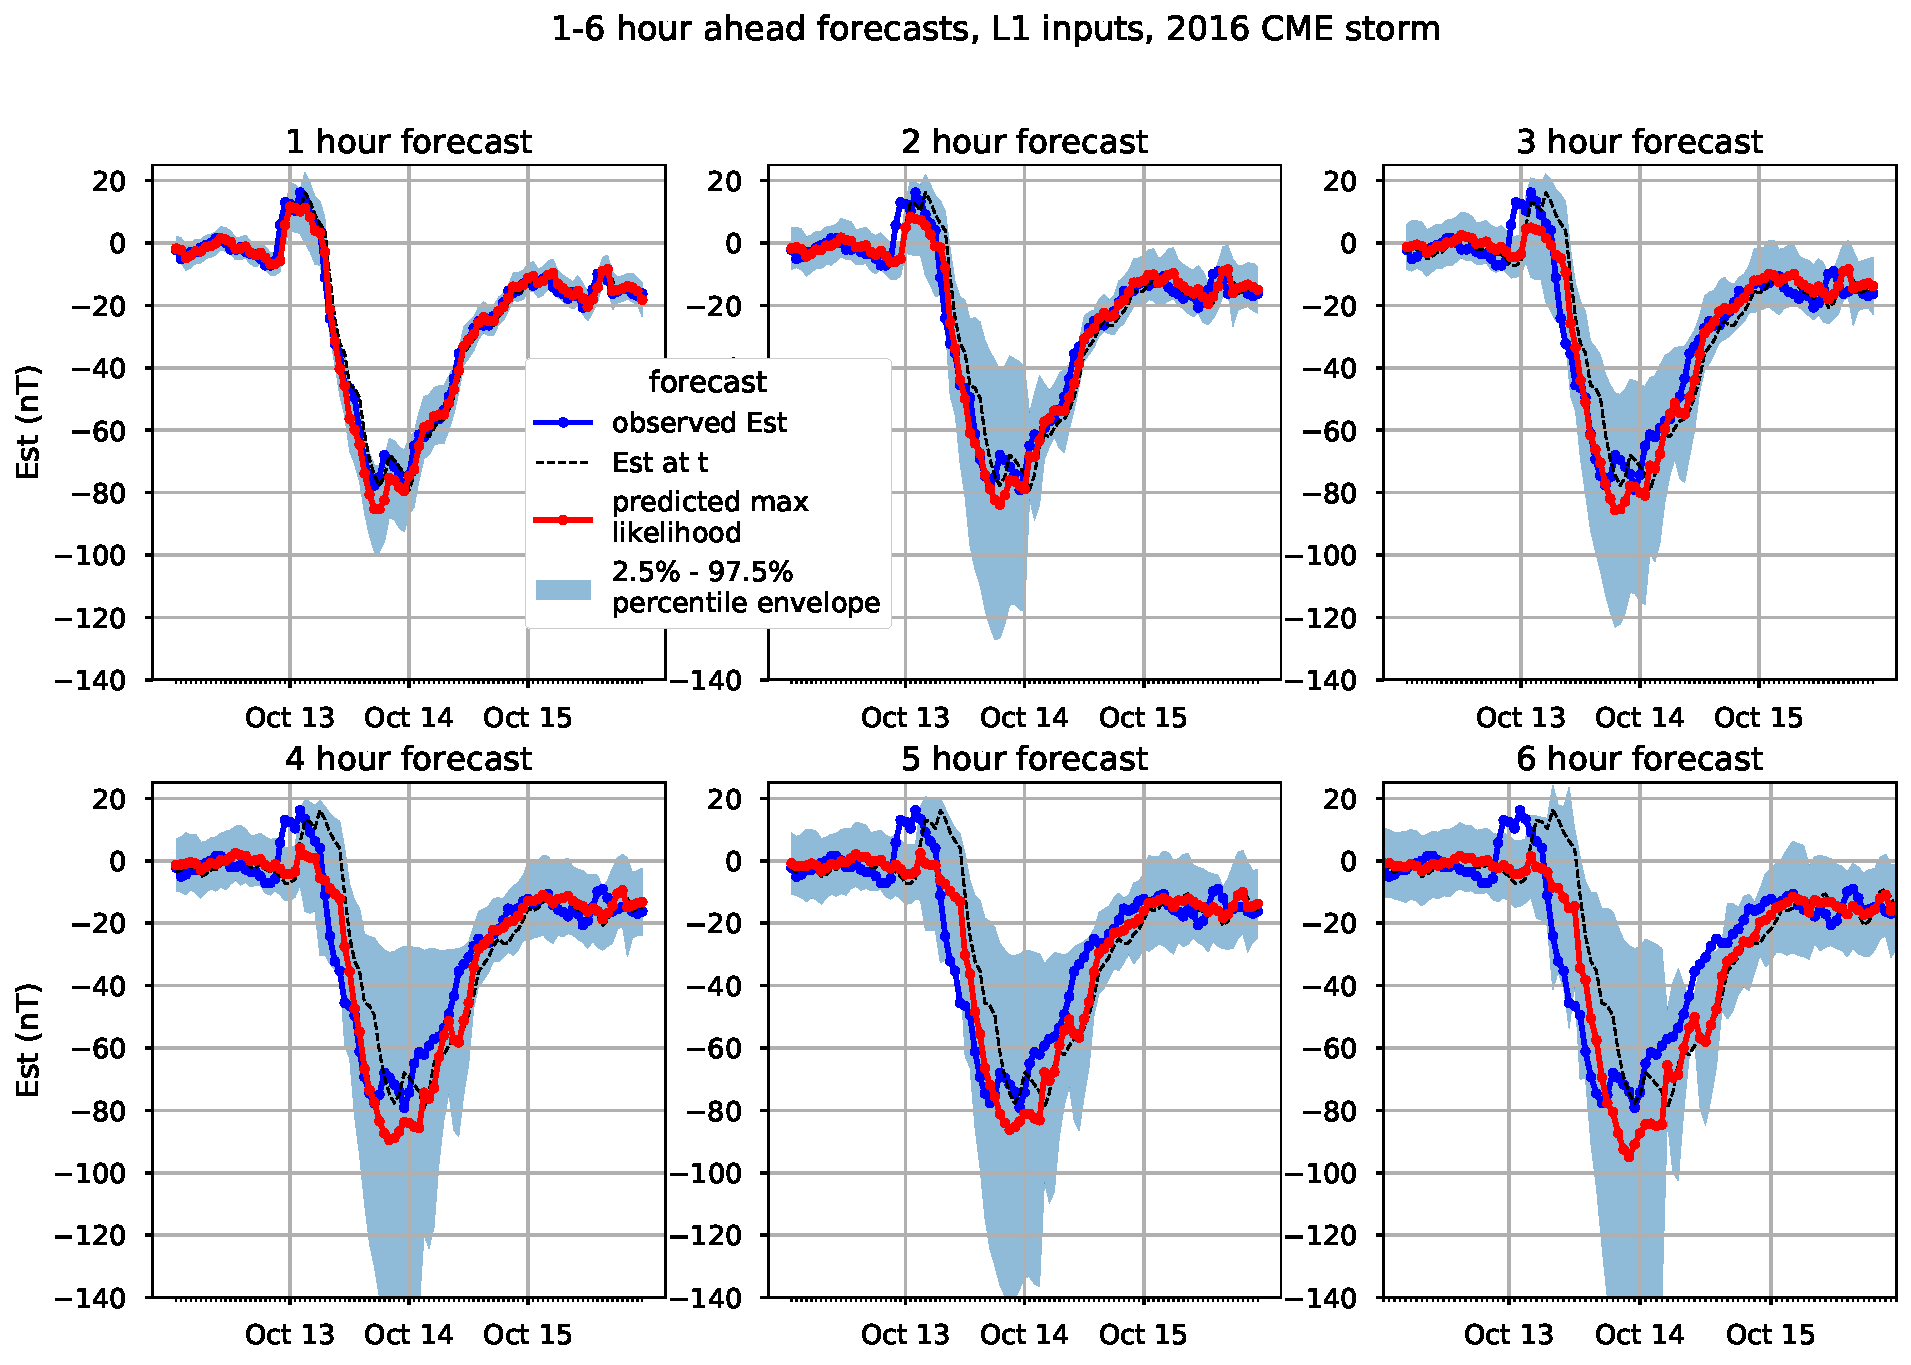
\includegraphics[width=1\textwidth]{figures/supplement/est_forecast_1-6_hour_L1_storm1.pdf}
   \caption{1-6 hour ahead forecasts for the 2016 CME storm for the networks with only observations from the L1 point as input.}
   \label{fig:storm1_l1}
\end{figure}

%%
%% LSTM
%%
\section*{Text S6: Long Short-Term Memory}

The complete set of equations for the LSTM is as follows
\begin{eqnarray*}
\mathbf{f}_t &= \sigma_g(W_f\,\mathbf{x}_t +U_f\,\mathbf{y}_{t-1} + \mathbf{b}_f) \\
\mathbf{i}_t &= \sigma_g(W_i\,\mathbf{x}_t + U_i\,\mathbf{y}_{t-1} + \mathbf{b}_i) \\
\mathbf{o}_t &= \sigma_g(W_o\,\mathbf{x}_t + U_o\,\mathbf{y}_{t-1} + \mathbf{b}_o) \\
\mathbf{c}_t &= \mathbf{f}_t \odot \mathbf{c}_{t-1} + \mathbf{i}_t \odot \sigma_h(W_c\,\mathbf{x}_t + \mathbf{U}_c\,\mathbf{y}_{t-1} + \mathbf{b}_c) \\
\mathbf{z}_t &= \mathbf{o}_t \odot \sigma_h(\mathbf{c}_t)
\end{eqnarray*}
which is then again combined with the input to generate a new output.
for input $\mathbf{x}_t \in \mathbb{R}^d$ at time $t$ and $\mathbf{z}, \mathbf{c} \in \mathbb{R}^m$ where $m$ is a hyperparameter defining the dimensionality of the cell memory $\mathbf{c}$ and output $\mathbf{z}$. The functions $\sigma_g(.)$ and $\sigma_h(.)$ are the sigmoid and hyperbolic tangent functions, respectively. The weights then have the following dimensions $W \in \mathbb{R}^{m\times d}$ and  $U \in \mathbb{R}^{m\times m}$ and the biases are all in $\mathbb{R}^m$. The $\odot$ operator signifies an elementwise product. Thus, for given dimensions $m$ and $d$, the total number of parameters to be learned within an LSTM cell is $4\,m\,d + 4\,m^2 + 4\,m$.

\section*{Other Supplementary Information}

\begin{figure}[htbp]
   \centering
   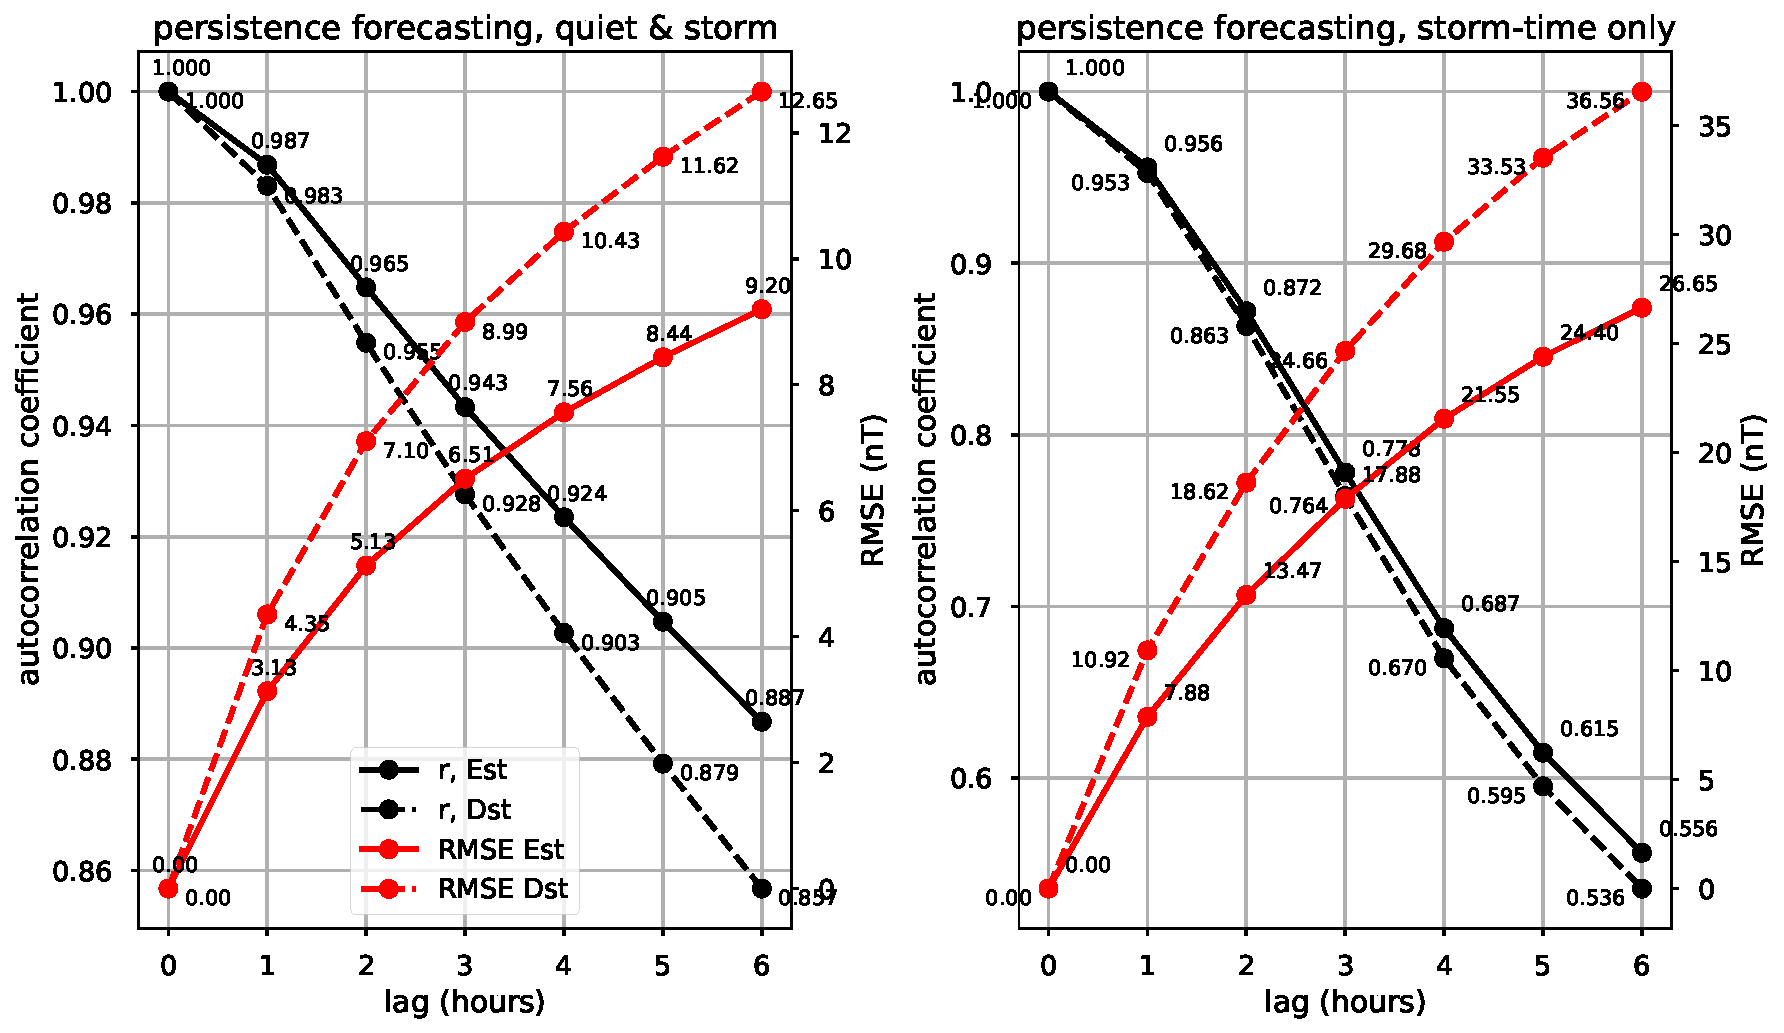
\includegraphics[width=1\textwidth]{figures/supplement/persistence.pdf}
   \caption{Pearson correlation coefficients and root mean squared errors of persistence forecasting of Est and Dst with lags up to 6 hours, demonstrating how persistence forecasting results in deceptively correlative and precise forecasts. On the left, forecasting is shown for all Est and Dst observations from 1996-2018, while on the right, storm-time observations have been isolated for persistence forecasting.}
   \label{fig:persistence}
\end{figure}

\begin{figure}[htbp]
  \centering
  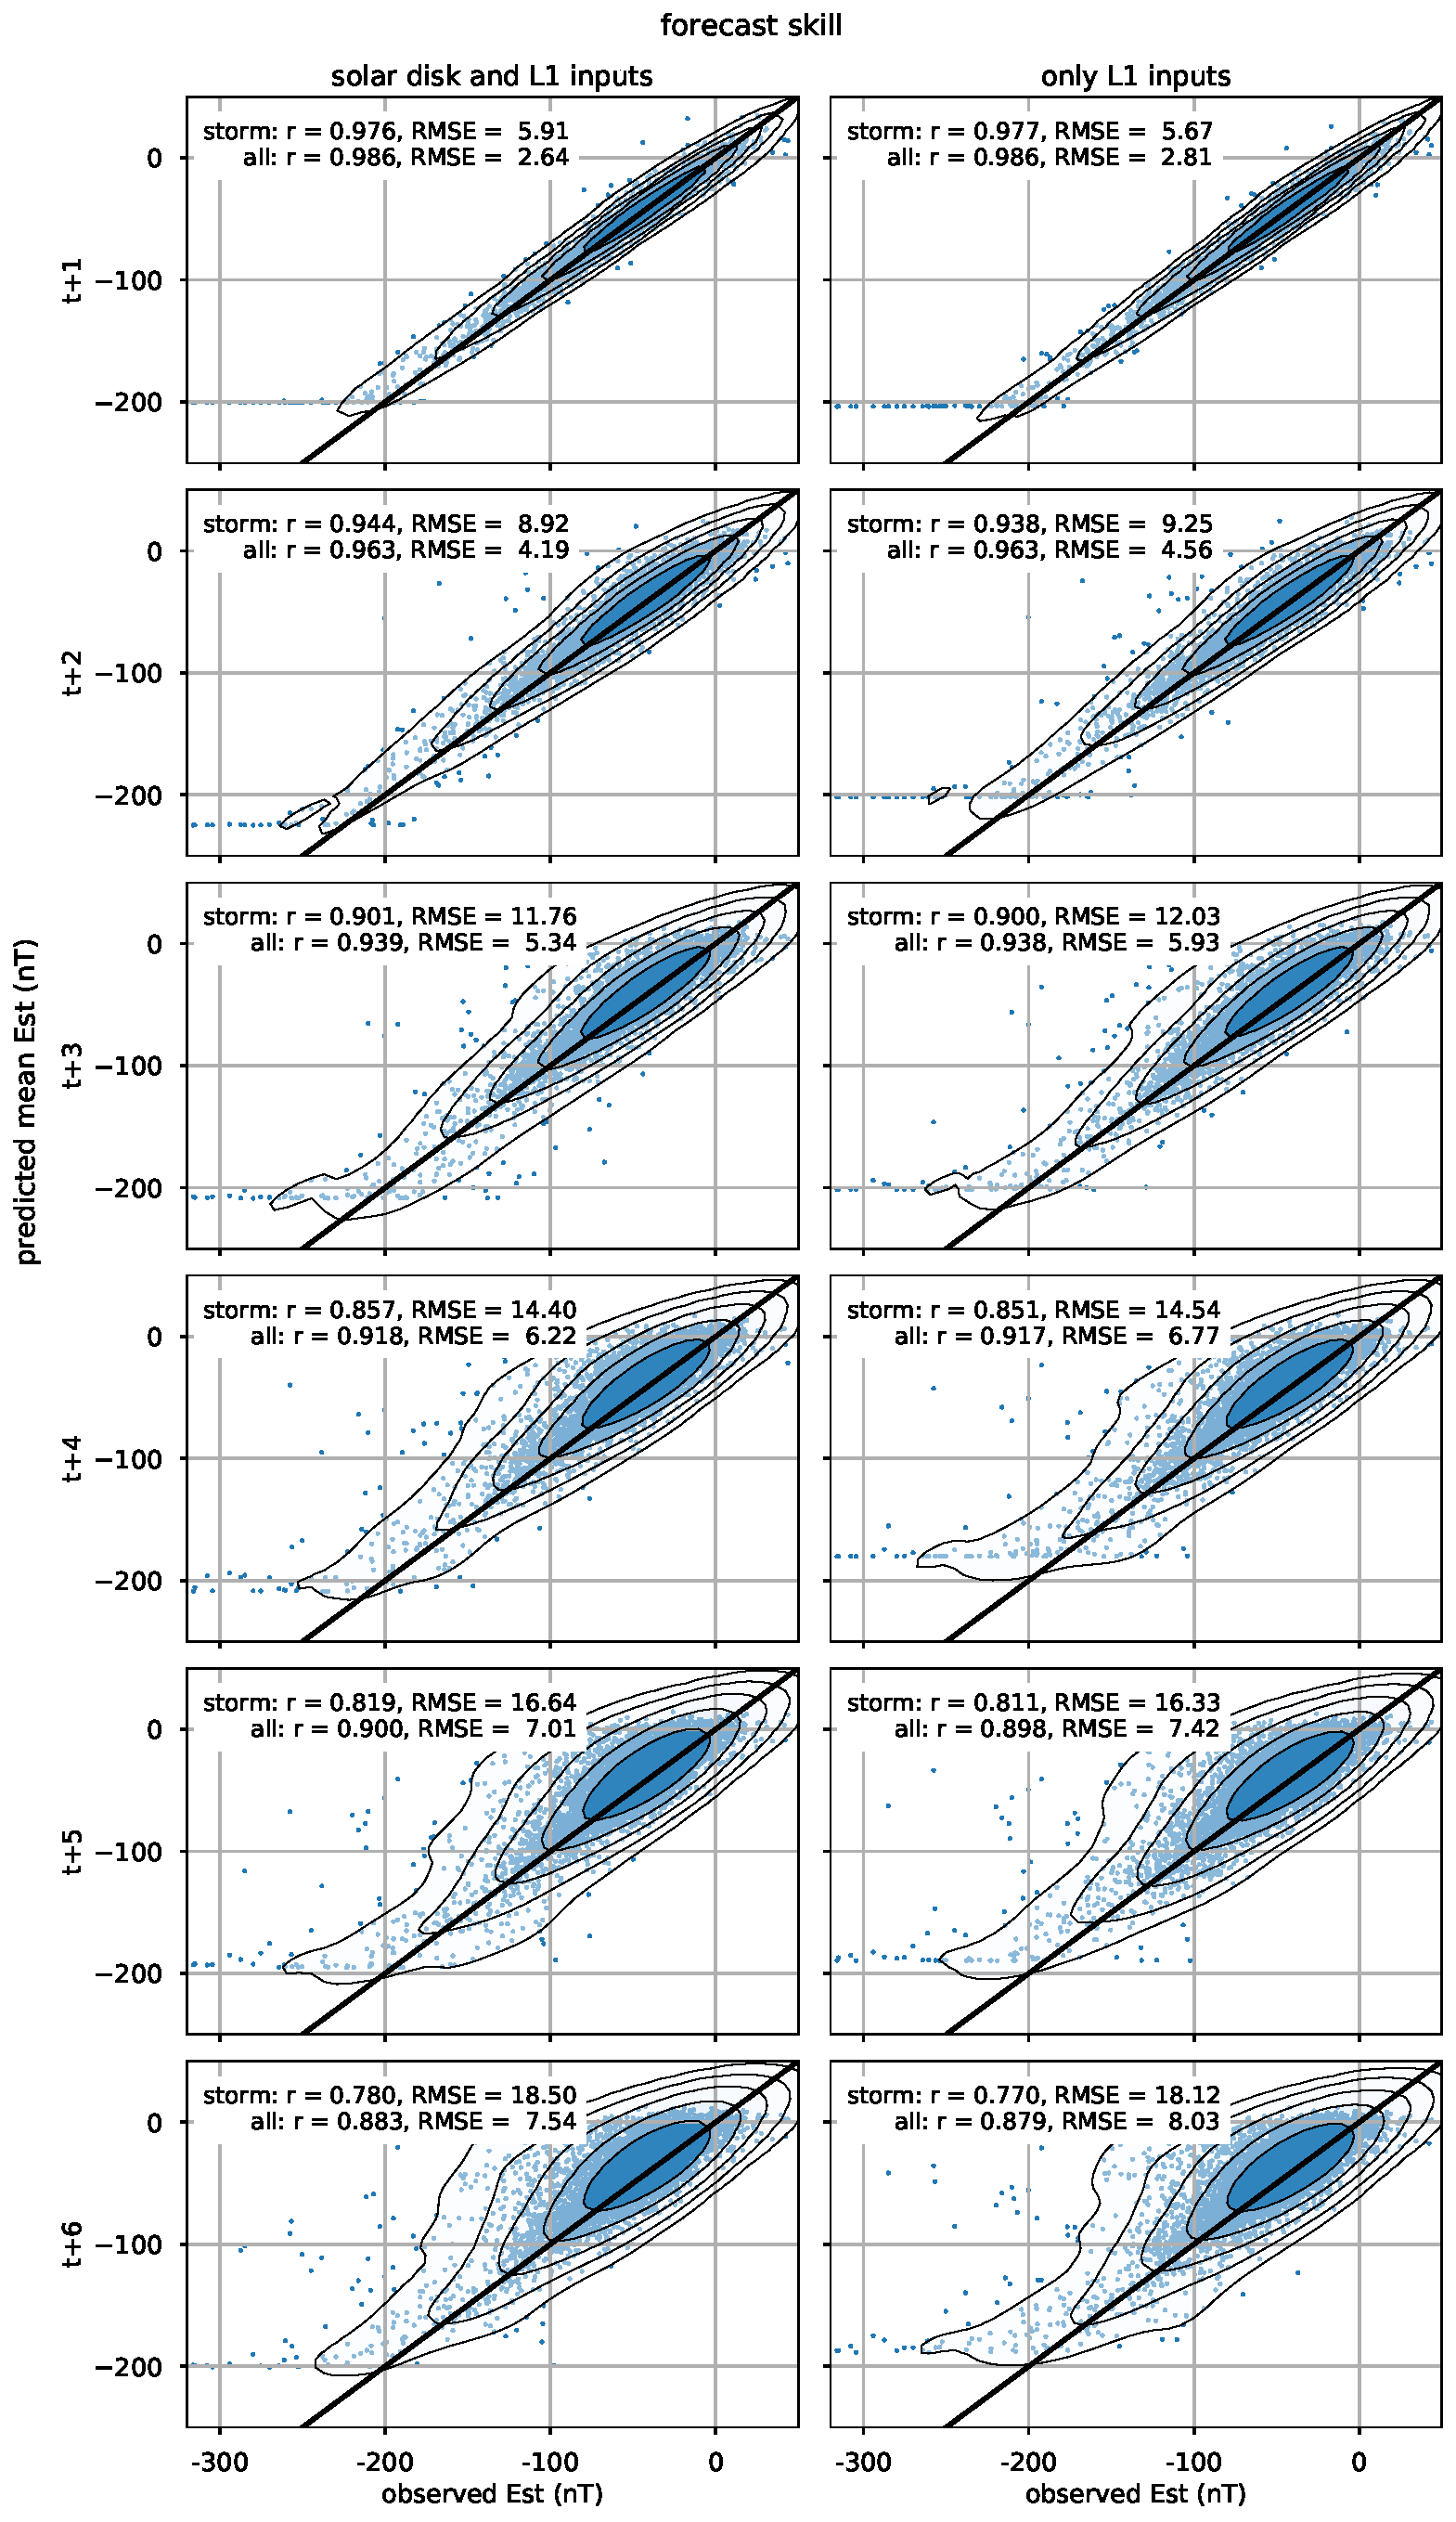
\includegraphics[width=0.8\textwidth]{figures/supplement/scatter.pdf} 
  \caption{Conventional forecast-observation scatter plots for both networks (in columns) and forecasts from one to six hours ahead (in rows). Points shown are for all storms from 1996-2018, including 5 hours before and after each storm. Contours, which are logarithmically spaced, show the Gaussian kernel density estimate for the point cloud to aid in visualizing data density. Also listed are typical skill values, namely the Pearson correlation coefficient and root mean square error (RMSE), which are computed separately for storm times and for all training and testing data.}
  \label{fig:scatter}
\end{figure}

\begin{table}[htpb]
\centering
\scriptsize
\begin{tabular}{l p{2.5cm} l l p{2.5cm} p{0.8cm} l}
Ahead & Architecture & R & RMSE (nT) & Inputs &  Database & Reference \\ \hline \hline
t + 1 & MLP, BP & 0.92 & 15 & n, v, Bz & 1963--1983 & \cite{Gleisner1996} \\ \hline
t + 1 & Elman Recurrent, BP  & 0.91 & 16 & n, v, Bz & 1963--1987 & \cite{Wu1996} \\ \hline
t + 1 & \multirow{8}{2.5cm}{Elman Recurrent, BP} & 0.91 & 14.5 & \multirow{8}{2.5cm}{n, v, Bx, By, Bz} & \multirow{8}{0.8cm}{1963--1992} & \multirow{8}{*}{\cite{Wu1997a}}  \\ 
t + 2 &   & 0.89 & 16.3 &&  &  \\
t + 3 &   & 0.86 & 18.2 &&  & \\
t + 4 &   & 0.83 & 19.9 &&  &\\
t + 5 &   & 0.82 & 20 &&  &\\
t + 6 &   & 0.82 & 20.8 &&  &\\
t + 7 &   & 0.80 & 21.8 &&  &\\
t + 8 &   & 0.77 & 23.1 && &\\ \hline
t + 1 & MLP, BP & 0.95 & 11 & n, v, Bx, By, Bz & 1972--1982 & \cite{Kugblenu1999} \\ \hline
t + 1 & Elman Recurrent, BP  & 0.88 &  & n, v, B, Bs & 1968--1987 & \cite{Munsami2000} \\ \hline
t + 1 & \multirow{8}{2.5cm}{MLP, BP}  & 0.95 &  & \multirow{8}{*}{previous Dst} & \multirow{8}{0.8cm}{1983} & \multirow{8}{*}{\cite{Stepanova2000}}  \\
t + 2 &  & 0.93 &  &&  & \\
t + 3 &  & 0.88 &  &&  & \\
t + 4 &  & 0.85 &  &&  & \\
t + 5 &  & 0.82 &  &&  & \\
t + 6 &  & 0.78 &  &&  & \\
t + 7 &  & 0.75 &  &&  & \\
t + 8 &  & 0.72 &  &&  & \\ \hline
t + 1 & \multirow{4}{2.5cm}{MLP, BP} & 0.93 &  & \multirow{4}{2.5cm}{Bx, By, Bz, B, n, v, dBx/dt, dBy/dt,
dBz/dt, dv/dt, dn/dt}& \multirow{4}{0.8cm}{1998--1999} &  \multirow{4}{*}{\cite{Jankovivcova2002}} \\
t + 6 &  & 0.73 &  &&  &  \\
t + 12 &  & 0.69 &  &&  &  \\
t + 18 &  & 0.66 &  &&  & \\ \hline
t + 1 & MLP, BP & 0.70 &  & polar cap index, previous Dst & 1997 & \cite{Stepanova2005} \\ \hline
t + 1 & Elman Recurrent, BP & 0.83 & 13.9 & By, Bz, B & 1995--2005 & \cite{Pallocchia2006} \\ \hline
t + 1 & \multirow{4}{2.5cm}{Locally Linear Neuro-Fuzzy Model} & 0.983 & 4.38 & \multirow{4}{2cm}{n, v, Bs, Dst, dDst/dt} &  \multirow{4}{0.8cm}{1995--1999} &  \multirow{4}{*}{\cite{Sharifie2006}} \\ 
t + 2 &  & 0.951 & 7.43 &&  & \\
t + 3 &  & 0.909 & 10 &&  &  \\
t + 4 &  & 0.870 & 11.83 && & \\ \hline
t + 1 & Radial Basis Function Network &  & 18.45 & n, v, Bs & 1998 & \cite{Wei2007} \\ \hline
t + 1 & \multirow{3}{2.5cm}{MLP, BP} & 0.86 & 8.84 & \multirow{3}{2.5cm}{Boyle index, Dp} &  \multirow{3}{0.8cm}{1998--2009}  & \multirow{3}{*}{\cite{Bala2012}} \\
t + 3 &  & 0.84 & 9.40 &&  & \\
t + 6 &  & 0.80 & 10.34 &&  &  \\ \hline
t + 1 & MLP, BP & 0.77 &  & Bz, n, v, T& 1998--2005 & \cite{Revallo2014} \\ \hline
t + 1 & Relevance Vector Machine & 0.96 & 10 & By, Bz, v, n, a:p, T, f10.7 & 1996--2007 & \cite{Andriyas2015} \\ \hline
t + 1 & \multirow{6}{2.5cm}{MLP, Particle Swarm} & 0.978 & 3.57 & \multirow{6}{2.5cm}{previous Dst}&  \multirow{6}{0.8cm}{1990--2016} &  \multirow{6}{*}{\cite{Lazzus2017}} \\
t + 2 &  & 0.936 & 5.97 & & &  \\
t + 3 &  & 0.895 & 7.54 && &  \\
t + 4 &  & 0.857 & 8.82 && &  \\
t + 5 &   & 0.825 & 9.75 && &  \\
t + 6 &  & 0.788 & 10.89 && &  \\ \hline
t + 1 & \multirow{6}{*}{LSTM, BP} & 0.966 & 5.25 & \multirow{6}{2.5cm}{n, v, B, Bz, B-GPS, previous Dst} &  \multirow{6}{0.8cm}{2001--2016} &  \multirow{6}{*}{\cite{Gruet2018}} \\
t + 2 &  & 0.946 & 6.55 &&  &  \\
t + 3 &  & 0.928 & 7.59 &&  &  \\
t + 4 &  & 0.910 & 8.53 &&  &  \\
t + 5 &  & 0.892 & 9.18 &&  &  \\
t + 6 &  & 0.873 & 9.86 &&  &  \\ \hline
t + 1 & \multirow{6}{*}{LSTM} & 0.986 & 2.64 & \multirow{6}{2.5cm}{Bx, By, Bz, n, v, T, lat, lon, CME (width, speed, accel, mass, energy), x-ray flux} & \multirow{6}{0.8cm}{1996--2018} &  \multirow{6}{*}{this study} \\
t + 2 &  & 0.963 & 4.19 & & & \\
t + 3 &  & 0.939 & 5.34 & & & \\ 
t + 4 &  & 0.918 & 6.22 & & & \\ 
t + 5 &  & 0.900 & 7.01 & & & \\ 
t + 6 &  & 0.883 & 7.54 & & & \\
\end{tabular}
\normalsize
\caption{Results of previous applications of neural networks to Dst forecasting, after \cite{Lazzus2017}. MLP: multilayered perceptron. BP: backpropagation. LSTM: long short-term memory. n: solar wind density. v: solar wind  velocity. a:p: alpha-to-proton ratio. Bs: southward-only component of interplanetary magnetic field. Dp: dynamic pressure = nv$^2$. Compare the values for $R$ and $RMSE$ with those resulting from a simple persistence forecast shown in Figure~\ref{fig:persistence}.}
\label{tab:prevNN}
\end{table}

%%Enter Data Set, Movie, and Audio captions here
%%EXAMPLE CAPTIONS

% \section*{Data Set S1.} %Type or paste caption here.

% Upload your dataset(s) to AGU's journal submission site and select
% "Supporting Information (SI)" as the file type. Following naming
% convention: ds01.

% Repeat for any additional Supporting data sets
\clearpage
\bibliography{refs.bib}

\end{document}